% Scout: one Postgres database, exposed through MCP to any AI chat session.
% Build: pdflatex mcp.tex
\documentclass[tikz,border=14pt]{standalone}
\usepackage{lmodern}
\usetikzlibrary{positioning,arrows.meta,fit,backgrounds}

\definecolor{ink}{HTML}{1F2328}
\definecolor{muted}{HTML}{6E7781}
\definecolor{line}{HTML}{8C959F}
\definecolor{accent}{HTML}{336791}  % Postgres blue
\definecolor{fill}{HTML}{F6F8FA}

\tikzset{
  >={Stealth[length=5pt,width=4pt]},
  every node/.style={font=\small, text=ink},
  box/.style={draw=line, fill=fill, rounded corners=3pt, line width=0.5pt,
              minimum height=10mm, inner xsep=8pt, align=center},
  db/.style={box, draw=accent, line width=1pt, fill=white, minimum width=36mm, minimum height=22mm},
  client/.style={box, fill=white, minimum width=30mm, minimum height=8mm},
  note/.style={font=\scriptsize, text=muted, align=center},
  flow/.style={->, draw=line, line width=0.6pt},
}

\begin{document}
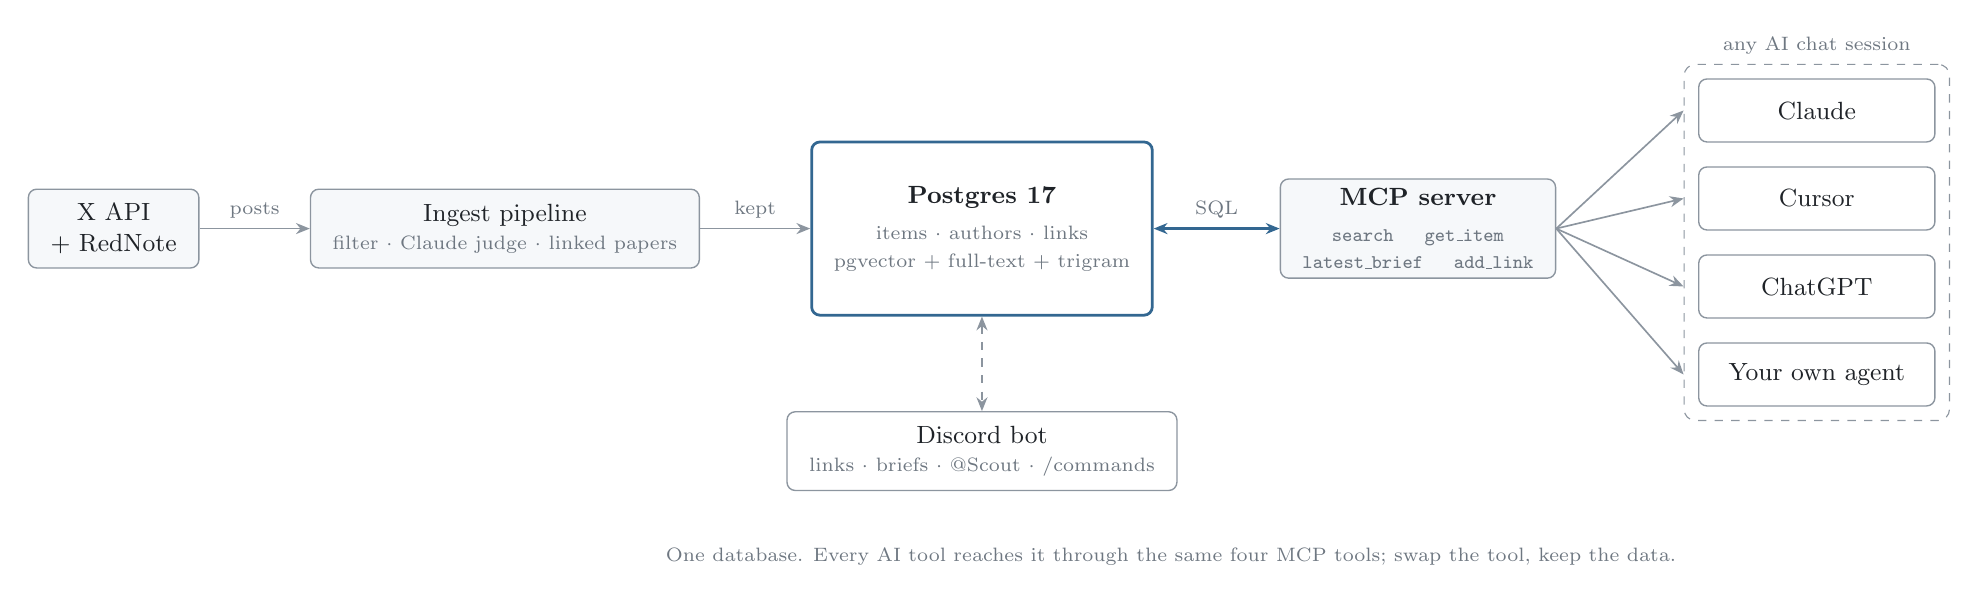
\begin{tikzpicture}[node distance=9mm and 14mm]

  % --- write side ---
  \node[box] (x) {X API\\ + RedNote};
  \node[box, right=of x] (pipe) {Ingest pipeline\\[-1pt]
    {\scriptsize\color{muted} filter $\cdot$ Claude judge $\cdot$ linked papers}};

  % --- the database ---
  \node[db, right=of pipe] (pg) {\textbf{Postgres 17}\\[2pt]
    {\scriptsize\color{muted} items $\cdot$ authors $\cdot$ links}\\[-1pt]
    {\scriptsize\color{muted} pgvector $+$ full-text $+$ trigram}};

  % --- the MCP server ---
  \node[box, right=16mm of pg, minimum width=34mm] (mcp) {\textbf{MCP server}\\[2pt]
    {\scriptsize\ttfamily\color{muted} search \ \ get\_item}\\[-1pt]
    {\scriptsize\ttfamily\color{muted} latest\_brief \ \ add\_link}};

  % --- any AI chat session ---
  \node[client, right=18mm of mcp, yshift=15mm] (c1) {Claude};
  \node[client, below=3mm of c1] (c2) {Cursor};
  \node[client, below=3mm of c2] (c3) {ChatGPT};
  \node[client, below=3mm of c3] (c4) {Your own agent};

  \begin{scope}[on background layer]
    \node[draw=line, dashed, rounded corners=4pt, inner sep=5pt,
          fit=(c1)(c4), label={[note]above:any AI chat session}] (clients) {};
  \end{scope}

  % --- arrows ---
  \draw[flow] (x) -- node[note, above] {posts} (pipe);
  \draw[flow] (pipe) -- node[note, above] {kept} (pg);
  \draw[<->, draw=accent, line width=0.8pt] (pg) -- node[note, above] {SQL} (mcp);
  \foreach \c in {c1,c2,c3,c4}
    \draw[->, draw=line, line width=0.6pt] (mcp.east) -- (clients.west |- \c.west);

  % --- Discord: the first front end, same database ---
  \node[box, below=12mm of pg, fill=white] (discord) {Discord bot\\[-1pt]
    {\scriptsize\color{muted} links $\cdot$ briefs $\cdot$ @Scout $\cdot$ /commands}};
  \draw[<->, draw=line, dashed, line width=0.6pt] (pg) -- (discord);

  % --- caption ---
  \node[note, below=6mm of discord, xshift=24mm] {One database. Every AI tool reaches it through the same four MCP tools; swap the tool, keep the data.};

\end{tikzpicture}
\end{document}
